\tikzstyle{inner} = [thin, circle, minimum size = 0.3cm, draw, inner sep = 0.1pt, black]
\tikzstyle{inner_g} = [thin, circle, minimum size = 0.3cm, draw, inner sep = 0.1pt, black, fill = green]
\tikzstyle{inner_r} = [thin, circle, minimum size = 0.3cm, draw, inner sep = 0.1pt, black, fill = red]
\tikzstyle{inner_b} = [thin, circle, minimum size = 0.3cm, draw, inner sep = 0.1pt, black, fill = blue!50!white]
\tikzstyle{ed} = [thick, ->, draw, black]

    
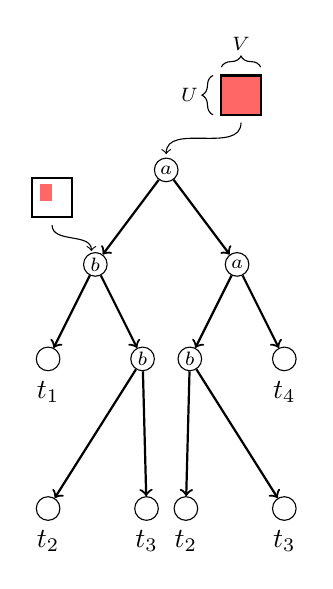
\begin{tikzpicture}
    \node[inner] (a) at (0, 0) {\scriptsize $a$};
    \node[inner] (b) at (-0.9, -1.2) {\scriptsize $b$};
    \node[inner] (c) at (0.9, -1.2) {\scriptsize $a$};
    \node[inner, label = below:$t_1$] (d) at (-1.5, -2.4) {};
    \node[inner] (e) at (-0.3, -2.4) {\scriptsize $b$};
    \node[inner] (e2) at (0.3, -2.4) {\scriptsize $b$};    
    \node[inner, label = below:$t_4$] (f) at (1.5, -2.4) {};
    \node[inner, label = below:$t_2$] (g) at (-1.5, -4.3) {};
    \node[inner, label = below:$t_3$] (h) at (-0.25, -4.3) {};
    \node[inner, label = below:$t_3$] (g2) at (1.5, -4.3) {};
    \node[inner, label = below:$t_2$] (h2) at (0.25, -4.3) {};

    
    \path (a) edge[ed] (b);
    \path (a) edge[ed] (c);
    \path (b) edge[ed] (d);
    \path (b) edge[ed] (e);
    \path (c) edge[ed] (e2);
    \path (c) edge[ed] (f);
    \path (e) edge[ed] (g);
    \path (e) edge[ed] (h);
    \path (e2) edge[ed] (g2);
    \path (e2) edge[ed] (h2);

    \draw[thick, black, fill = red!60!white] (0.7, 1.2) rectangle (1.2, 0.7);
    \draw [black, decorate, decoration = {brace, amplitude = 4pt}, xshift = -3pt] (0.7, 0.7) -- (0.7, 1.2)
	    node [black, midway, xshift = -0.3cm] {\scriptsize $U$};
    \draw [black, decorate, decoration = {brace, amplitude = 4pt}, yshift = 3pt] (0.7, 1.2) -- (1.2, 1.2)
    	node [black, midway, yshift = 0.3cm] {\scriptsize $V$};
    \draw[->] (0.95, 0.6) to[out = 270, in = 90] (0, 0.2);

    \draw[thick, black] (-1.7, -0.1) rectangle (-1.2, -0.6);
    \fill[red!60!white] (-1.6, -0.18) rectangle (-1.45, -0.4);
    \draw[->] (-1.45, -0.7) to[out = 270, in = 90] (-0.95, -1.03);
\end{tikzpicture}
